%----------------------------------------------------------------------------------------
%	PACKAGES AND THEMES
%----------------------------------------------------------------------------------------
\documentclass[aspectratio=169,xcolor=dvipsnames]{beamer}
\usetheme{SimplePlus}

\usepackage{hyperref}
\usepackage{graphicx} % Allows including images
\usepackage{booktabs} % Allows the use of \toprule, \midrule and \bottomrule in tables
\usepackage[UTF8]{ctex}
\usepackage{url}
\usepackage{listings}
\usepackage{graphics}
\usepackage{mathtools}
\usepackage{booktabs}
\usepackage{xcolor}
%----------------------------------------------------------------------------------------
%	TITLE PAGE
%----------------------------------------------------------------------------------------

\title[]{排序} % The short title appears at the bottom of every slide, the full title is only on the title page
% \subtitle{Subtitle}

\author[Ziqi Zhao] {zziqi229@gmail.com}

\institute[NTU] % Your institution as it will appear on the bottom of every slide, may be shorthand to save space
{
    % Department of Computer Science and Information Engineering \\
    % National Taiwan University % Your institution for the title page
}
\date{\today} % Date, can be changed to a custom date

\begin{document}

\begin{frame}
    \titlepage
\end{frame}

\begin{frame}{主题}
    \begin{enumerate}
        \item 选择排序
        \item 插入排序
        \item 冒泡排序
        \item 归并排序
        \item 如何使用快速排序
    \end{enumerate}
\end{frame}

\begin{frame}{选择排序}
    \begin{enumerate}
        \item 首先在未排序序列中找到最小元素,存放到排序序列的末尾位置
        \item 再从剩余未排序元素中继续寻找最小元素,然后放到已排序序列的末尾
        \item 重复以上的步骤,直到未排序序列为空。
    \end{enumerate}
\end{frame}

\begin{frame}{选择排序}
    \begin{itemize}
        \item 3 5 4 1 2
        \item \textcolor{red}{3} 5 4  \textcolor{red}{1} 2 $\rightarrow$ \textcolor{red}{1} 5 4  \textcolor{red}{3} 2
        \item \textcolor{blue}{1} \textcolor{red}{5} 4 3 \textcolor{red}{2} $\rightarrow$ \textcolor{blue}{1} \textcolor{red}{2} 4 3 \textcolor{red}{5}
        \item \textcolor{blue}1 \textcolor{blue}2 \textcolor{red}4 \textcolor{red}3 5 $\rightarrow$ \textcolor{blue}1 \textcolor{blue}2 \textcolor{red}3 \textcolor{red}4 5
        \item \textcolor{blue}1 \textcolor{blue}2 \textcolor{blue}3 \textcolor{red}4 5
        \item \textcolor{blue}1 \textcolor{blue}2 \textcolor{blue}3 \textcolor{blue}4 \textcolor{red}5
        \item \textcolor{blue}1 \textcolor{blue}2 \textcolor{blue}3 \textcolor{blue}4 \textcolor{blue}5
    \end{itemize}

\end{frame}

\begin{frame}{冒泡排序}
    \begin{enumerate}
        \item 比较相邻的元素。如果第一个比第二个大,就交换他们两个。
        \item 对每一对相邻元素作同样的工作,从开始第一对到结尾的最后一对。这步做完后,最后的元素会是最大的数。
        \item 针对所有的元素重复以上的步骤,除了最后一个。
        \item 持续每次对越来越少的元素重复上面的步骤,直到没有任何一对数字需要比较。
    \end{enumerate}
\end{frame}

\begin{frame}{冒泡排序 round 1}
    \begin{itemize}
        \item 4 6 3 1 5 2
        \item 4 \textcolor{red}{6 3} 1 5 2 $\rightarrow$ 4 \textcolor{red}{3 6} 1 5 2
        \item 4 3 \textcolor{red}{6 1} 5 2 $\rightarrow$ 4 3 \textcolor{red}{1 6} 5 2
        \item 4 3 1 \textcolor{red}{6 5} 2 $\rightarrow$ 4 3 1 \textcolor{red}{5 6} 2
        \item 4 3 1 5 \textcolor{red}{6 2} $\rightarrow$ 4 3 1 5 \textcolor{red}{2 6}
    \end{itemize}
\end{frame}

\begin{frame}{冒泡排序 round 2}
    \begin{itemize}
        \item 4 3 1 5 2 \textcolor{blue}{6}
        \item \textcolor{red}{4 3} 1 5 2 \textcolor{blue}{6} $\rightarrow$ \textcolor{red}{3 4} 1 5 2 \textcolor{blue}{6}
        \item 3 \textcolor{red}{4 1} 5 2 \textcolor{blue}{6} $\rightarrow$ 3 \textcolor{red}{1 4} 5 2 \textcolor{blue}{6}
        \item 3 1 \textcolor{red}{4 5} 2 \textcolor{blue}{6}
        \item 3 1 4 \textcolor{red}{5 2} \textcolor{blue}{6} $\rightarrow$ 3 1 4 \textcolor{red}{2 5} \textcolor{blue}{6}
        \item 3 1 4 2 \textcolor{blue}{5 6}
    \end{itemize}
\end{frame}

\begin{frame}{冒泡排序 round 3}
    \begin{itemize}
        \item 3 1 4 2 \textcolor{blue}{5 6}
        \item \textcolor{red}{3 1} 4 2 \textcolor{blue}{5 6} $\rightarrow$ \textcolor{red}{1 3} 4 2 \textcolor{blue}{5 6}
        \item 1 \textcolor{red}{3 4} 2 \textcolor{blue}{5 6}
        \item 1 3 \textcolor{red}{4 2} \textcolor{blue}{5 6} $\rightarrow$ 1 3 \textcolor{red}{2 4} \textcolor{blue}{5 6}
        \item 1 3 2 \textcolor{blue}{4 5 6}
    \end{itemize}
\end{frame}

\begin{frame}{冒泡排序 round 4}
    \begin{itemize}
        \item 1 3 2 \textcolor{blue}{4 5 6}
        \item \textcolor{red}{1 3} 2 \textcolor{blue}{4 5 6}
        \item 1 \textcolor{red}{3 2} \textcolor{blue}{4 5 6} $\rightarrow$ 1 \textcolor{red}{2 3} \textcolor{blue}{4 5 6}
        \item 1 2 \textcolor{blue}{3 4 5 6} 
    \end{itemize}
\end{frame}

\begin{frame}{冒泡排序 round 5}
    \begin{itemize}
        \item 1 2 \textcolor{blue}{3 4 5 6}
        \item \textcolor{red}{1 2} \textcolor{blue}{3 4 5 6}
        \item \textcolor{blue}{1 2 3 4 5 6}
    \end{itemize}
\end{frame}

\begin{frame}{插入排序}
    \begin{enumerate}
        \item 序列分为已排序序列和未排序序列
        \item 从左到右扫描每一个元素,将第 $i$ 个元素插入到已序序列中适当的位置
    \end{enumerate}
\end{frame}


\begin{frame}{归并排序}
    \begin{enumerate}
        \item 如果序列长度为1,则已经有序
        \item 将序列氛围左右两半序列,问题分解为规模较小的相同问题,递归知道序列长度为1
        \item 问题变为将两个有序序列$A,B$合并
        \item 设置两个位置$p1$,$p2$,当$A[p1] \le A[p2]$ 将$A[p1]$ 加入序列$C$末尾,否则将 $A[p2]$加入C末尾
    \end{enumerate}
\end{frame}


\begin{frame}{归并排序}
    \centering{ 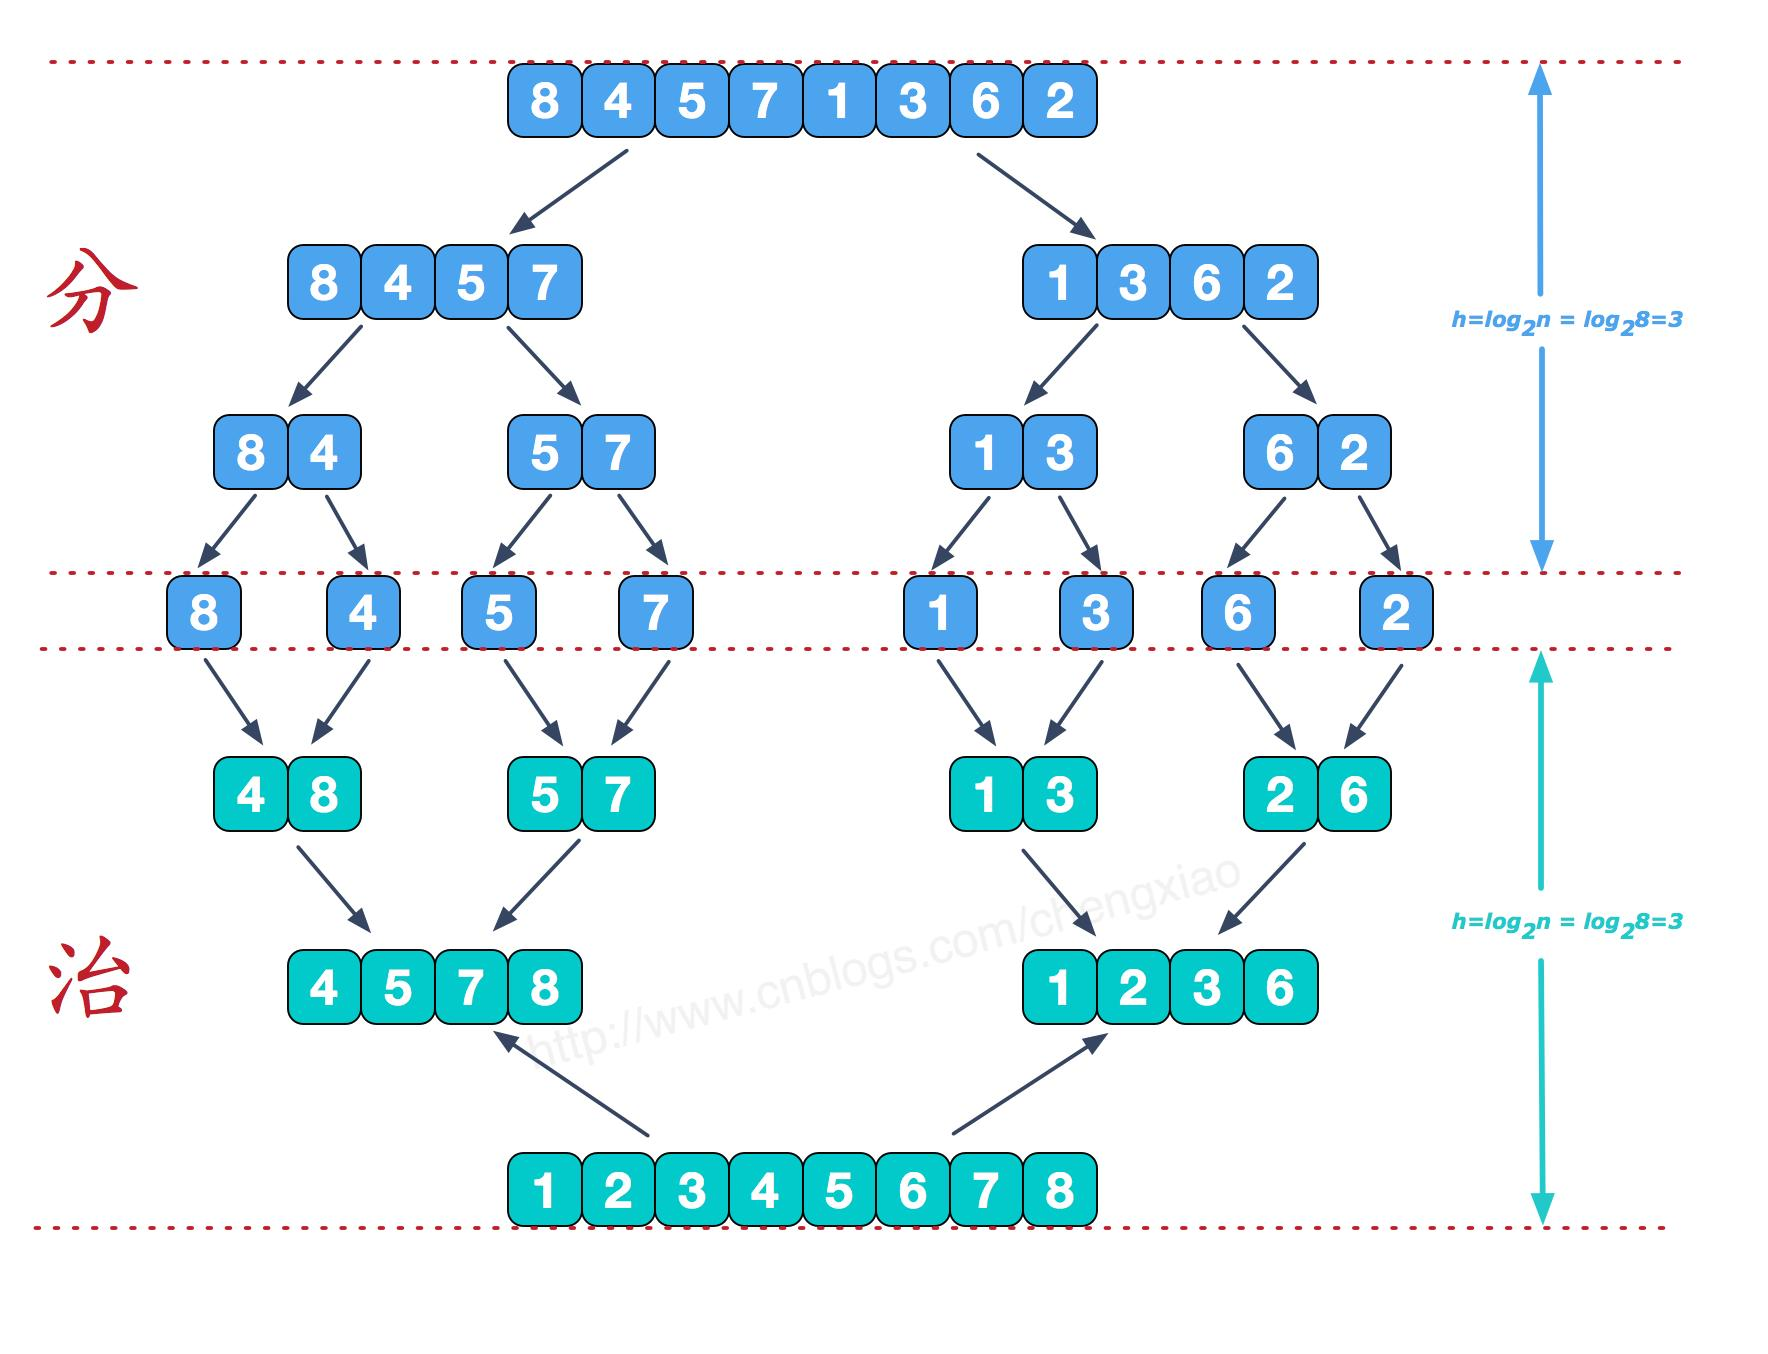
\includegraphics[scale=0.34]{merge/merge1.jpg}}
\end{frame}

\begin{frame}
    \frametitle{\href{https://www.luogu.com.cn/problem/P1177}{luoguP1177 【模板】排序}}

    第一行输入一个数字 $n, n \le 10^5 $\\
    第二行输入$n$个空格隔开的正整数,从小到大排序后输出
\end{frame}

% \begin{frame}{Python}
%     \begin{block}{}
%         n = int(input())\\
%         s = input().split()\\
%         w = [int(i) for i in s]\\
%         w.sort()\\
%         for i in w:\\
%         \quad print(i, end=' ')\\
%     \end{block}
% \end{frame}


% \begin{frame}{cpp}
%     \begin{block}{}
%         const int maxn = 1e5 + 5;
%         int n;
%         int w[maxn];
%         int main() {
%         \quad ios::sync_with_stdio(false);
%         \quad cin >> n;
%         \quad for (int i = 1; i <= n; i++)
%         \quad \quad cin >> w[i];
%         \quad sort(w + 1, w + 1 + n);
%         \quad for (int i = 1; i <= n; i++)
%         \quad \quad cout << w[i] << " ";
%         \quad return 0;
%         }
%     \end{block}
% \end{frame}


% \begin{frame}{Java}
%     \begin{block}{}

%     \end{block}
% \end{frame}

\begin{frame}{\href{https://www.luogu.com.cn/problem/P1093}{luoguP1093 奖学金}}

\end{frame}

\begin{frame}{\href{https://www.luogu.com.cn/problem/P1223}{luoguP1223 排队接水}}
    有 $n$ 个人在一个水龙头前排队接水,假如每个人接水的时间为 $T_i$\\
    请找出这 $n$ 个人排队的一种顺序,使得 $n$个人的平均等待时间最小。
\end{frame}


\end{document}
